% Options for packages loaded elsewhere
\PassOptionsToPackage{unicode}{hyperref}
\PassOptionsToPackage{hyphens}{url}
%
\documentclass[
]{book}
\usepackage{amsmath,amssymb}
\usepackage{lmodern}
\usepackage{ifxetex,ifluatex}
\ifnum 0\ifxetex 1\fi\ifluatex 1\fi=0 % if pdftex
  \usepackage[T1]{fontenc}
  \usepackage[utf8]{inputenc}
  \usepackage{textcomp} % provide euro and other symbols
\else % if luatex or xetex
  \usepackage{unicode-math}
  \defaultfontfeatures{Scale=MatchLowercase}
  \defaultfontfeatures[\rmfamily]{Ligatures=TeX,Scale=1}
\fi
% Use upquote if available, for straight quotes in verbatim environments
\IfFileExists{upquote.sty}{\usepackage{upquote}}{}
\IfFileExists{microtype.sty}{% use microtype if available
  \usepackage[]{microtype}
  \UseMicrotypeSet[protrusion]{basicmath} % disable protrusion for tt fonts
}{}
\makeatletter
\@ifundefined{KOMAClassName}{% if non-KOMA class
  \IfFileExists{parskip.sty}{%
    \usepackage{parskip}
  }{% else
    \setlength{\parindent}{0pt}
    \setlength{\parskip}{6pt plus 2pt minus 1pt}}
}{% if KOMA class
  \KOMAoptions{parskip=half}}
\makeatother
\usepackage{xcolor}
\IfFileExists{xurl.sty}{\usepackage{xurl}}{} % add URL line breaks if available
\IfFileExists{bookmark.sty}{\usepackage{bookmark}}{\usepackage{hyperref}}
\hypersetup{
  pdftitle={Notas de Programación en R},
  pdfauthor={Rubén Fernández Casal (rubenfcasal@gmail.com)},
  hidelinks,
  pdfcreator={LaTeX via pandoc}}
\urlstyle{same} % disable monospaced font for URLs
\usepackage{color}
\usepackage{fancyvrb}
\newcommand{\VerbBar}{|}
\newcommand{\VERB}{\Verb[commandchars=\\\{\}]}
\DefineVerbatimEnvironment{Highlighting}{Verbatim}{commandchars=\\\{\}}
% Add ',fontsize=\small' for more characters per line
\usepackage{framed}
\definecolor{shadecolor}{RGB}{248,248,248}
\newenvironment{Shaded}{\begin{snugshade}}{\end{snugshade}}
\newcommand{\AlertTok}[1]{\textcolor[rgb]{0.94,0.16,0.16}{#1}}
\newcommand{\AnnotationTok}[1]{\textcolor[rgb]{0.56,0.35,0.01}{\textbf{\textit{#1}}}}
\newcommand{\AttributeTok}[1]{\textcolor[rgb]{0.77,0.63,0.00}{#1}}
\newcommand{\BaseNTok}[1]{\textcolor[rgb]{0.00,0.00,0.81}{#1}}
\newcommand{\BuiltInTok}[1]{#1}
\newcommand{\CharTok}[1]{\textcolor[rgb]{0.31,0.60,0.02}{#1}}
\newcommand{\CommentTok}[1]{\textcolor[rgb]{0.56,0.35,0.01}{\textit{#1}}}
\newcommand{\CommentVarTok}[1]{\textcolor[rgb]{0.56,0.35,0.01}{\textbf{\textit{#1}}}}
\newcommand{\ConstantTok}[1]{\textcolor[rgb]{0.00,0.00,0.00}{#1}}
\newcommand{\ControlFlowTok}[1]{\textcolor[rgb]{0.13,0.29,0.53}{\textbf{#1}}}
\newcommand{\DataTypeTok}[1]{\textcolor[rgb]{0.13,0.29,0.53}{#1}}
\newcommand{\DecValTok}[1]{\textcolor[rgb]{0.00,0.00,0.81}{#1}}
\newcommand{\DocumentationTok}[1]{\textcolor[rgb]{0.56,0.35,0.01}{\textbf{\textit{#1}}}}
\newcommand{\ErrorTok}[1]{\textcolor[rgb]{0.64,0.00,0.00}{\textbf{#1}}}
\newcommand{\ExtensionTok}[1]{#1}
\newcommand{\FloatTok}[1]{\textcolor[rgb]{0.00,0.00,0.81}{#1}}
\newcommand{\FunctionTok}[1]{\textcolor[rgb]{0.00,0.00,0.00}{#1}}
\newcommand{\ImportTok}[1]{#1}
\newcommand{\InformationTok}[1]{\textcolor[rgb]{0.56,0.35,0.01}{\textbf{\textit{#1}}}}
\newcommand{\KeywordTok}[1]{\textcolor[rgb]{0.13,0.29,0.53}{\textbf{#1}}}
\newcommand{\NormalTok}[1]{#1}
\newcommand{\OperatorTok}[1]{\textcolor[rgb]{0.81,0.36,0.00}{\textbf{#1}}}
\newcommand{\OtherTok}[1]{\textcolor[rgb]{0.56,0.35,0.01}{#1}}
\newcommand{\PreprocessorTok}[1]{\textcolor[rgb]{0.56,0.35,0.01}{\textit{#1}}}
\newcommand{\RegionMarkerTok}[1]{#1}
\newcommand{\SpecialCharTok}[1]{\textcolor[rgb]{0.00,0.00,0.00}{#1}}
\newcommand{\SpecialStringTok}[1]{\textcolor[rgb]{0.31,0.60,0.02}{#1}}
\newcommand{\StringTok}[1]{\textcolor[rgb]{0.31,0.60,0.02}{#1}}
\newcommand{\VariableTok}[1]{\textcolor[rgb]{0.00,0.00,0.00}{#1}}
\newcommand{\VerbatimStringTok}[1]{\textcolor[rgb]{0.31,0.60,0.02}{#1}}
\newcommand{\WarningTok}[1]{\textcolor[rgb]{0.56,0.35,0.01}{\textbf{\textit{#1}}}}
\usepackage{longtable,booktabs,array}
\usepackage{calc} % for calculating minipage widths
% Correct order of tables after \paragraph or \subparagraph
\usepackage{etoolbox}
\makeatletter
\patchcmd\longtable{\par}{\if@noskipsec\mbox{}\fi\par}{}{}
\makeatother
% Allow footnotes in longtable head/foot
\IfFileExists{footnotehyper.sty}{\usepackage{footnotehyper}}{\usepackage{footnote}}
\makesavenoteenv{longtable}
\usepackage{graphicx}
\makeatletter
\def\maxwidth{\ifdim\Gin@nat@width>\linewidth\linewidth\else\Gin@nat@width\fi}
\def\maxheight{\ifdim\Gin@nat@height>\textheight\textheight\else\Gin@nat@height\fi}
\makeatother
% Scale images if necessary, so that they will not overflow the page
% margins by default, and it is still possible to overwrite the defaults
% using explicit options in \includegraphics[width, height, ...]{}
\setkeys{Gin}{width=\maxwidth,height=\maxheight,keepaspectratio}
% Set default figure placement to htbp
\makeatletter
\def\fps@figure{htbp}
\makeatother
\setlength{\emergencystretch}{3em} % prevent overfull lines
\providecommand{\tightlist}{%
  \setlength{\itemsep}{0pt}\setlength{\parskip}{0pt}}
\setcounter{secnumdepth}{5}
\usepackage{booktabs}
\usepackage[a4paper, top=3.25cm, bottom=2.5cm, left=3cm, right=2.5cm]{geometry}
% \usepackage{fontspec}
% \setmainfont{Arial}
% \usepackage{amsthm}
% Espacio después de teorema
% Basado en https://tex.stackexchange.com/questions/37797/theorem-environment-line-break-after-label
% \newtheoremstyle{break}
%   {\topsep}{\topsep}% Space above and below
%   {\itshape}{}%       Body font, Indent amoun
%   {\bfseries}{}%      Theorem head font, Punctuation after theorem head
%   {\newline}%         Space after theorem head
%   {}%                 Theorem head spec (can be left empty, meaning ‘normal’ )
% Problemas con listas  https://tex.stackexchange.com/questions/8110/is-it-possible-to-skip-the-first-line-in-a-theorem-environment

\usepackage{ntheorem}
\theoremstyle{break}
\theoremheaderfont{\normalfont\bfseries}
\theorembodyfont{\normalfont}
\theorempreskip{\bigskipamount}
\theorempostskip{\smallskipamount}
\theoremprework{\bigskip\hrule\leavevmode}
\theoremseparator{\smallskip}
\theorempostwork{\bigskip\hrule\bigskip}
\newtheorem{theorem}{Teorema}[chapter]
\theoremprework{\bigskip\hrule\leavevmode}
\theorempostwork{\bigskip\hrule\bigskip}
\newtheorem{conjecture}{Algoritmo}[chapter]
\newtheorem{lemma}{Lema}[chapter]
\newtheorem{corollary}{Corolario}[chapter]
\newtheorem{proposition}{Proposición}[chapter]
\newtheorem{definition}{Definición}[chapter]
\newtheorem{hypothesis}{Hipótesis}[chapter]
\newtheorem{exercise}{Ejercicio}[chapter]
%\theoremprework{\bigskip\leavevmode}
%\theorempostwork{\vspace*{-\bigskipamount}\vspace*{-\medskipamount}}
\newtheorem{example}{Ejemplo}[chapter]
\theoremstyle{nonumberplain}
\theoremheaderfont{\normalfont\itshape}
\theoremseparator{:}
% \theorempostwork{\hrule}
\newtheorem{remark}{Nota}
\newtheorem{solution}{Solución}
\newtheorem{proof}{Demostración}


\ifxetex
  \usepackage{polyglossia}
  \setmainlanguage{spanish}
  % Tabla en lugar de cuadro
  \gappto\captionsspanish{\renewcommand{\tablename}{Tabla}
          \renewcommand{\listtablename}{Índice de tablas}}

\else
  \usepackage[spanish,es-tabla]{babel}
\fi
\makeatletter
\def\thm@space@setup{%
  \thm@preskip=8pt plus 2pt minus 4pt
  \thm@postskip=\thm@preskip
}
\makeatother
\ifluatex
  \usepackage{selnolig}  % disable illegal ligatures
\fi
\usepackage[]{natbib}
\bibliographystyle{apalike}

\title{Notas de Programación en R}
\author{Rubén Fernández Casal (\href{mailto:rubenfcasal@gmail.com}{\nolinkurl{rubenfcasal@gmail.com}})}
\date{Edición: Marzo de 2023. Impresión: 2023-03-29}

\begin{document}
\maketitle

{
\setcounter{tocdepth}{1}
\tableofcontents
}
\hypertarget{pruxf3logo}{%
\chapter*{Prólogo}\label{pruxf3logo}}
\addcontentsline{toc}{chapter}{Prólogo}

Este es un libro, \textbf{\emph{en proceso de elaboración}}, con notas personales sobre programación en R para el análisis de datos, en el que incluyen referencias a información y recursos adicionales (se asumen unos conocimientos básicos de R).
El contenido está sesgado por la experiencia personal (es mi forma de programar en R) pero puede resultar útil para otras personas.
Cualquier sugerencia de mejora o comentario será bien recibido.

Este libro ha sido escrito en \href{http://rmarkdown.rstudio.com}{R-Markdown} empleando el paquete \href{https://bookdown.org/yihui/bookdown/}{\texttt{bookdown}} y está disponible en el repositorio Github: \href{https://github.com/rubenfcasal/book_notasr}{rubenfcasal/book\_notasr}.
Se puede acceder a la versión en línea a través del siguiente enlace:

\url{https://rubenfcasal.github.io/book_notasr}.

donde puede descargarse en formato \href{https://rubenfcasal.github.io/book_notasr/Notas_R.pdf}{pdf}.

Para seguir los ejemplos mostrados en el libro se recomienda tener instalados los siguientes paquetes (realmente no se emplean todos):
\href{https://www.r-project.org}{\texttt{Rcmdr}}, \href{https://github.com/topepo/caret/}{\texttt{caret}}, \href{https://tidymodels.tidymodels.org}{\texttt{tidymodels}}, \href{https://tidyverse.tidyverse.org}{\texttt{tidyverse}}, \href{https://ycphs.github.io/openxlsx/index.html}{\texttt{openxlsx}}, \href{https://github.com/rstudio/DT}{\texttt{DT}}, \href{https://github.com/rstudio/rmarkdown}{\texttt{rmarkdown}}, \href{https://yihui.org/knitr/}{\texttt{knitr}}, \href{https://remotes.r-lib.org}{\texttt{remotes}}, \href{https://devtools.r-lib.org/}{\texttt{devtools}}.
Por ejemplo mediante los siguientes comandos:

\begin{Shaded}
\begin{Highlighting}[]
\NormalTok{pkgs }\OtherTok{\textless{}{-}} \FunctionTok{c}\NormalTok{(}\StringTok{"Rcmdr"}\NormalTok{, }\StringTok{"caret"}\NormalTok{, }\StringTok{"tidymodels"}\NormalTok{, }\StringTok{"tidyverse"}\NormalTok{, }\StringTok{"openxlsx"}\NormalTok{, }\StringTok{"DT"}\NormalTok{, }
          \StringTok{"rmarkdown"}\NormalTok{, }\StringTok{"knitr"}\NormalTok{, }\StringTok{"remotes"}\NormalTok{, }\StringTok{"devtools"}\NormalTok{)}
\FunctionTok{install.packages}\NormalTok{(}\FunctionTok{setdiff}\NormalTok{(pkgs, }\FunctionTok{installed.packages}\NormalTok{()[,}\StringTok{"Package"}\NormalTok{]), }\AttributeTok{dependencies =} \ConstantTok{TRUE}\NormalTok{)}
\end{Highlighting}
\end{Shaded}

(puede que haya que seleccionar el repositorio de descarga, e.g.~\emph{Oficina de software libre (CIXUG)}).

El código anterior no reinstala los paquetes ya instalados, por lo que podrían aparecer problemas debidos a incompatibilidades entre versiones (aunque no suele ocurrir, salvo que nuestra instalación de R esté muy desactualizada).
Si es el caso, en lugar de la última línea se puede ejecutar:

\begin{Shaded}
\begin{Highlighting}[]
\FunctionTok{install.packages}\NormalTok{(pkgs, }\AttributeTok{dependencies =} \ConstantTok{TRUE}\NormalTok{) }\CommentTok{\# Instala todos...}
\end{Highlighting}
\end{Shaded}

Para generar el libro (compilar) serán necesarios paquetes adicionales,
para lo que se recomendaría consultar el libro de \href{https://rubenfcasal.github.io/bookdown_intro}{``Escritura de libros con bookdown''} en castellano.

Este obra está bajo una licencia de \href{https://creativecommons.org/licenses/by-nc-nd/4.0/deed.es_ES}{Creative Commons Reconocimiento-NoComercial-SinObraDerivada 4.0 Internacional}
(esperamos poder liberarlo bajo una licencia menos restrictiva más adelante\ldots).


\includegraphics[width=1.22in]{by-nc-nd-88x31}

\hypertarget{intro}{%
\chapter{Introducción}\label{intro}}

Como aparece en el prólogo, estos apuntes contienen recomendaciones y notas personales sobre programación en R para el análisis de datos, en el que incluyen referencias a información y recursos adicionales que considero de interés.
Se tratará de mostrar una forma de llevar a cabo las distintas tareas que pueden surgir en el análisis de datos empleando R, esto no quiere decir que sea la mejor forma de hacerlo o la más cómoda (que dependerá de cada persona).

En estas notas \textbf{\emph{se asumen unos conocimientos básicos de R}}, un lenguaje de programación (interpretado) y un entorno estadístico desarrollado específicamente para el análisis estadístico.
Puede ser una herramienta de gran utilidad a lo largo de todo el proceso de obtención de información a partir de datos (ver Figura \ref{fig:esquema}).

\begin{figure}[!htb]

{\centering 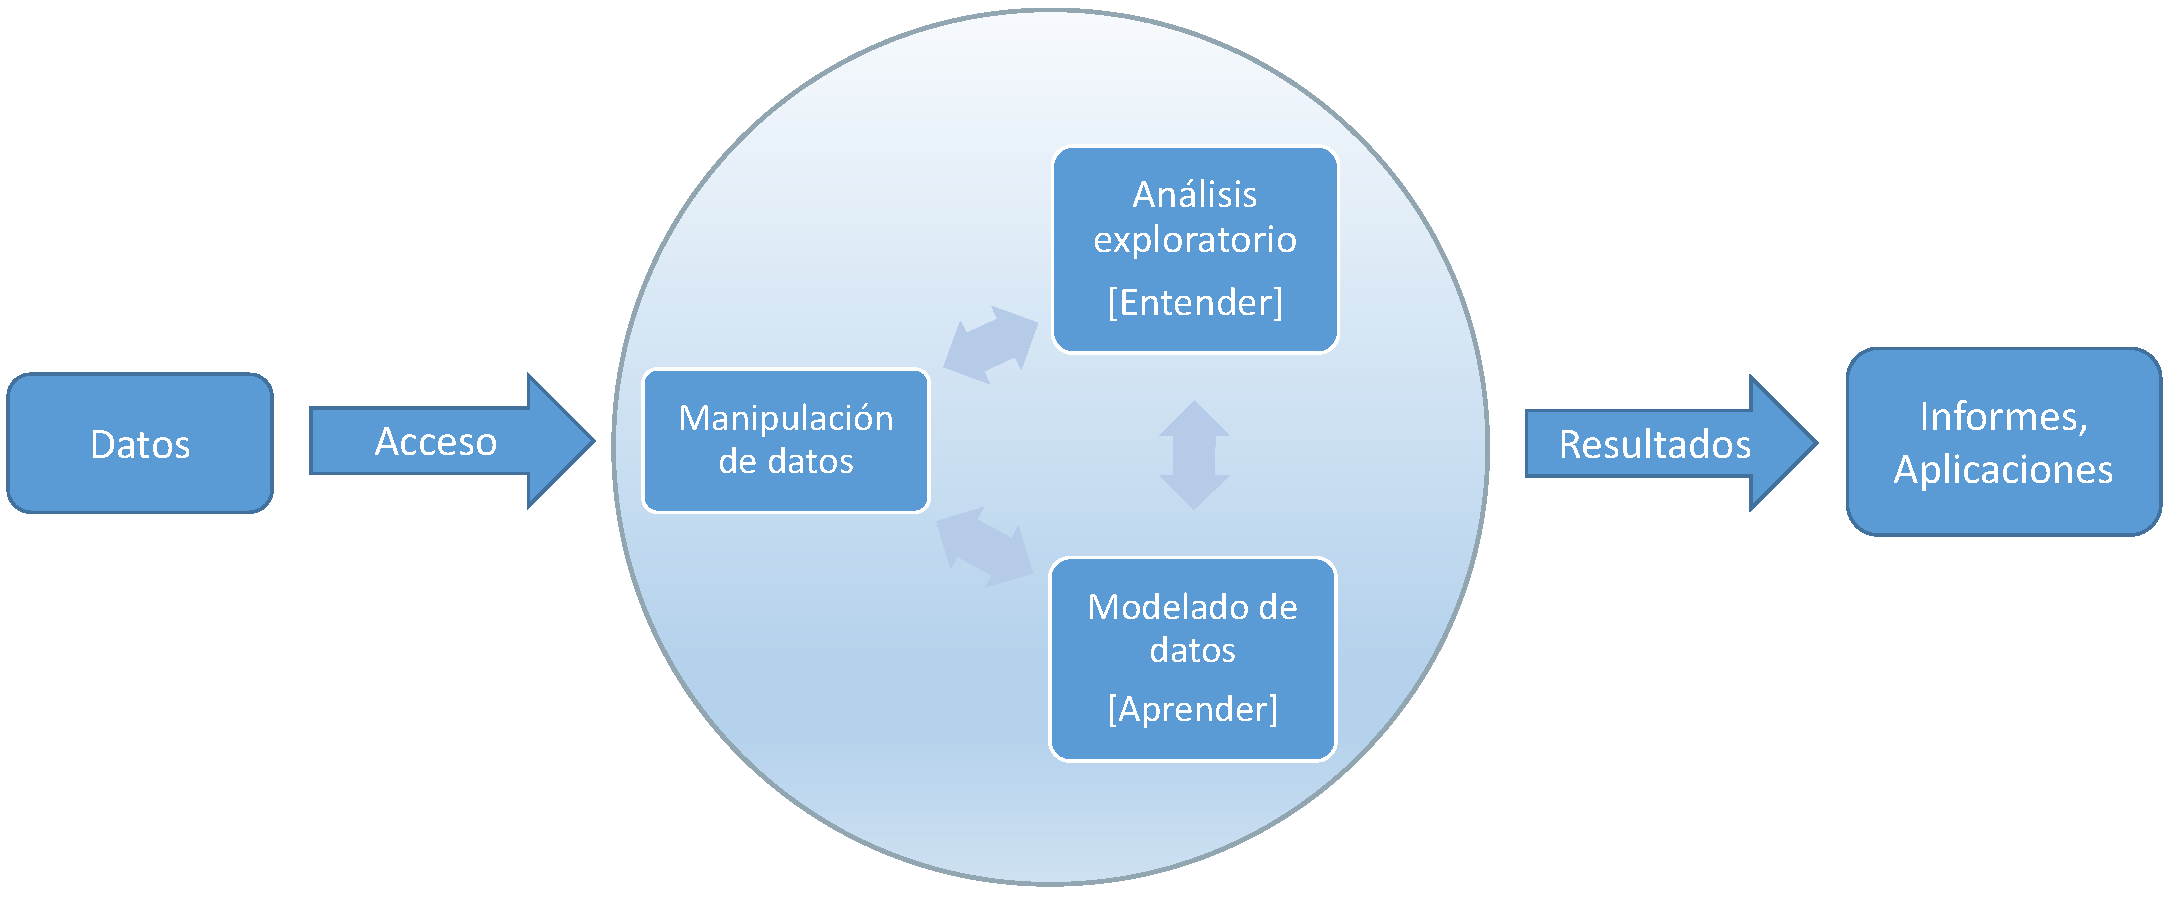
\includegraphics[width=0.8\linewidth]{figuras/esquema2} 

}

\caption{Etapas del proceso}\label{fig:esquema}
\end{figure}

Para una introducción a la programación en R se puede consultar el libro:

Fernández-Casal R., Roca-Pardiñas J., Costa J. y Oviedo-de la Fuente M. (2022). \emph{\href{https://rubenfcasal.github.io/intror}{Introducción al Análisis de Datos con R}} (\href{https://github.com/rubenfcasal/intror}{github}).

Adicionalmente, en este \href{https://rubenfcasal.github.io/post/ayuda-y-recursos-para-el-aprendizaje-de-r}{post} se incluyen enlaces a recursos adicionales, incluyendo libros y cursos, que pueden ser útiles para el aprendizaje de R.

El primer paso es la instalación de R, para ello se recomienda seguir los pasos en este \href{https://rubenfcasal.github.io/post/instalacion-de-r}{post}.

Para el desarrollo de código e informes la recomendación es emplear \emph{RStudio Desktop}, que se puede instalar y configurar siguiendo las indicaciones en este \href{https://rubenfcasal.github.io/post/instalacion-de-rstudio}{post}.
También puede resultar de interés consultar:

\begin{itemize}
\item
  \href{https://posit.co/wp-content/uploads/2022/10/rstudio-ide-1.pdf}{RStudio cheatsheet}
\item
  \href{https://support.posit.co/hc/en-us/sections/200107586-Using-the-RStudio-IDE}{Using the RStudio IDE}
\end{itemize}

Sin embargo, en ciertos casos puede ser recomendable ejecutar el código R directamente desde una ventana de comandos (por ejemplo para ejecutar varios programas de forma simultánea en distintos directorios de trabajo o si los requerimientos computacionales son grandes).
En mi caso, cuando trabajo en Windows, acostumbro a emplear el explorador para situarme en el directorio donde quiero ejecutar código y abrir una ventana de comandos, escribiendo \texttt{cmd} en el cuadro superior donde se muestra la ruta.
Posteriormente, como añadí en directorio de instalación de R al \emph{path} (ver \href{https://rubenfcasal.github.io/post/instalacion-de-r/\#rtools}{post}), ejecuto\footnote{También se puede ejecutar un script de R de forma no interactiva ejecutando en el intérprete de comandos del sistema operativo: \texttt{R\ CMD\ BATCH\ {[}opciones{]}\ mi\_script.R\ {[}fichero\_salida{]}} (cambiando \texttt{R} por la ruta completa, e.g.~\texttt{"C:\textbackslash{}Program\ Files\textbackslash{}R\textbackslash{}R-4.2.1\textbackslash{}bin\textbackslash{}R.exe"}, si no se añadió al path. También se puede incluir en un fichero \emph{.bat}, para poder ejecutarlo repetidas veces con mayor facilidad). Ver \href{https://cran.r-project.org/doc/manuals/r-release/R-intro.html\#Invoking-R}{Appendix B Invoking R} de \href{https://cran.r-project.org/doc/manuals/r-release/R-intro.html}{Introduction to R} para información sobre las distintas opciones.} \texttt{R} y finalmente un comando de la forma:

\begin{Shaded}
\begin{Highlighting}[]
\FunctionTok{source}\NormalTok{(}\StringTok{"mi\_script.R"}\NormalTok{, }\AttributeTok{echo =} \ConstantTok{TRUE}\NormalTok{, }\AttributeTok{encoding =} \StringTok{"UTF{-}8"}\NormalTok{) }\CommentTok{\# UTF{-}8 importante en R \textless{} 4.2}
\end{Highlighting}
\end{Shaded}

\hypertarget{organizacion}{%
\section{Organización}\label{organizacion}}

Para la organización de archivos (datos, código, informes\ldots) lo recomendable es emplear un directorio con la estructura adecuada.

Dependiendo del objetivo puede interesar emplear un proyecto de RStudio (menú \emph{File \textgreater{} New project\ldots{}}).
En mi caso empleo esta opción para paquetes, libros en bookdown, webs con blogdown y aplicaciones shiny.
En otros casos empleo una carpeta que puede tener subdirectorios (si el proyecto es más grande) para distintos tipos de archivos o para distintas tareas (con el objetivo de facilitar la búsqueda).
Por ejemplo: \emph{datos}, \emph{informes}, \emph{resultados\_2023}\ldots{}

Mi recomendación es emplear nombres de archivos y carpetas en minúscula (o con la primera letra en mayúsculas), sin espacios (por ejemplo empleando \texttt{\_} para separar palabras o iniciales) y sin caracteres especiales (ASCII, sin acentos\ldots).
Los nombres deberían ser lo más descriptivos posibles (en el sentido de evitar confusión).
Pueden incluirse descripciones más completas en el código, en ficheros de texto (e.g.~\emph{Descripcion\_archivos.txt}), o incluso en hojas de cálculo.
Yo además acostumbro a incluir archivos del tipo \emph{Notas.txt} (con recordatorios, decisiones\ldots) o \emph{Pendente.txt} (con próximos pasos, mejoras o verificaciones pendientes\ldots).

Además, nos puede interesar establecer opciones de R específicas para el proyecto (por ejemplo opciones de configuración de memoria, de paquetes o variables de entorno, incluyendo claves privadas), de forma que se establezcan automáticamente al iniciar R o RStudio.
Para más detalles ver la ayuda de \texttt{?Startup}, el apéndice \href{https://cran.r-project.org/doc/manuals/r-release/R-intro.html\#Invoking-R}{Invoking R} o el post de RStudio
\href{https://support.posit.co/hc/en-us/articles/360047157094-Managing-R-with-Rprofile-Renviron-Rprofile-site-Renviron-site-rsession-conf-and-repos-conf}{Managing R with .Rprofile, .Renviron, Rprofile.site, Renviron.site, rsession.conf, and repos.conf}

Para desarrollar código y proyectos de forma colaborativa, la recomendación es emplear un sistema de control de versiones.
Se puede configurar RStudio para emplear Git (ver el libro \href{https://happygitwithr.com/index.html}{Happy Git and GitHub for the useR} o la sección \href{https://r-pkgs.org/software-development-practices.html\#sec-sw-dev-practices-git-github}{Git and GitHub}), sin embargo yo prefiero emplear \href{https://desktop.github.com/}{GitHub Desktop}.

\hypertarget{codigo}{%
\subsection{Código e informes}\label{codigo}}

Mi recomendación a la hora de escribir código es seguir un \textbf{proceso iterativo}.
Se comienza realizando pruebas y al finalizar cada etapa se trata de reorganizar el código (adaptándolo al estilo de programación elegido, lo que incluiría añadir comentarios y secciones) de forma que sea más cómodo continuar trabajando en siguientes etapas (y si es posible que resulte más fácil de adaptar para otros casos).

En el caso de informes el proceso sería similar, empleando como punto de partida un fichero de código en formato \href{https://rubenfcasal.github.io/bookdown_intro/rmarkdown.html\#spin}{spin} (ver e.g.~\href{https://rubenfcasal.github.io/bookdown_intro/rmarkdown.html\#spin}{Apéndice}), en el que el texto RMarkdown se incluye como un comentario de código empleando \texttt{\#\textquotesingle{}}. Por ejemplo:

\begin{verbatim}
#' # Sección
#'
#' ## Subsección
#'
#' Texto rmarkdown...
\end{verbatim}

En primer lugar me preocupo de escribir un código funcional y, además de ir añadiendo comentarios de la forma habitual, voy añadiendo secciones y texto rmarkdown en formato spin.
Finalmente, cuando tengo una primera versión del código (que puedo ir previsualizando; en RStudio basta con pulsar\footnote{Para mostrar las combinaciones de teclas en RStudio podemos emplear el menú \emph{Tools \textgreater{} Keyboard Shortcuts Help}.} \emph{Ctrl + Shift + K}, el icono correspondiente en la barra superior, o seleccionar \emph{File \textgreater{} Compile Report\ldots{}}), lo transformo a formato \emph{.Rmd} con un comando de la forma:

\begin{Shaded}
\begin{Highlighting}[]
\NormalTok{knitr}\SpecialCharTok{::}\FunctionTok{spin}\NormalTok{(}\StringTok{"Informe.R"}\NormalTok{, }\AttributeTok{knit =} \ConstantTok{FALSE}\NormalTok{)}
\end{Highlighting}
\end{Shaded}

donde termino de redactar (\texttt{knitr::purl("Informe.Rmd",\ documentation\ =\ 2)} genera un nuevo fichero \emph{Informe.R} donde resulta más cómodo modificar o desarrollar código).

Se recomienda \textbf{elegir un estilo que sea consistente y seguirlo por completo} en todo el proyecto.
Lo principal sería el operador de asignación, el espaciado y el estilo de nombres (de objetos, variables o ficheros):

\begin{itemize}
\item
  \texttt{estilo.clasico}: es el estilo del paquete base de R. Muchos programadores no lo recomiendan (principalmente porque este separador no se admite en otros lenguajes y porque puede dar lugar a confusión con métodos S3, ver Sección \ref{oop}).
\item
  \texttt{estilo\_serpiente} (o \texttt{Estilo\_serpiente}): es el estilo de la colección de paquetes \href{https://tidyverse.tidyverse.org}{\texttt{tidyverse}}.
\item
  \texttt{EstiloCamello} (o \texttt{estiloCamello}): es el estilo (casi obligatorio) para las clases \href{https://r6.r-lib.org}{\texttt{R6}} (ver Sección \ref{oop}). El paquete \href{https://shiny.rstudio.com/}{\texttt{shiny}} emplea la variante que comienza por minúsculas.
\end{itemize}

\textbf{Recomiendo emplear \texttt{\textless{}-}} como operador de asignación y escribir todos los \textbf{nombres en minúsculas}.
Yo tengo tendencia a emplear el \texttt{estilo.clasico}, sobre todo si el código no depende de paquetes tidyverse (en ese caso suelo emplear \texttt{estilo\_serpiente}).
También influye el estilo de nombres empleado por la fuente de datos o el requerido en los resultados.

El estilo también debe especificar el sangrado, el espaciado, etc.
Por ejemplo:

\begin{itemize}
\item
  \href{https://style.tidyverse.org}{Tidyverse style guide}
\item
  \href{https://google.github.io/styleguide/Rguide.html}{Google's R Style Guide}
\end{itemize}

Para facilitar la legibilidad \textbf{es muy recomendable incluir un espacio} entre los elementos del comando.
En RStudio se puede seleccionar un trozo de (una línea de) código y pulsar \emph{Ctrl + Shift + A} para formatearlo.
También podemos emplear el paquete \href{https://github.com/r-lib/styler}{\texttt{styler}} para formatear el código.
Por ejemplo, en RStudio podemos emplear \emph{Addins \textgreater{} Styler \textgreater{} Style active file}.

Además se recomienda \textbf{crear secciones y documentar el código adecuadamente}.
En RStudio se puede crear una sección pulsando \emph{Ctrl + Shift + R} o añadiendo al menos 4 guiones (\texttt{-}, también \texttt{=} o \texttt{\#}) después de un comentario.
Por ejemplo:

\begin{Shaded}
\begin{Highlighting}[]
\CommentTok{\# Sección {-}{-}{-}{-}}
\DocumentationTok{\#\# Subsección {-}{-}{-}{-}}
\end{Highlighting}
\end{Shaded}

El orden de las secciones y subsecciones es importante.
Al principio del código debería ir:

\begin{enumerate}
\def\labelenumi{\arabic{enumi}.}
\tightlist
\item
  Los parámetros o variables globales.
\item
  La carga de paquetes (únicamente los mínimos requeridos).
\item
  La carga de código externo.
\item
  La carga de archivos de datos (o al principio de la sección donde se emplean, si son datos auxiliares).
\end{enumerate}

\textbf{No se recomienda} emplear rutas absolutas en el código, del tipo:

\begin{Shaded}
\begin{Highlighting}[]
\FunctionTok{setwd}\NormalTok{(}\StringTok{"C:/Documentos/Proyectos/Proyecto\_X"}\NormalTok{)}
\FunctionTok{load}\NormalTok{(}\StringTok{"C:/Documentos/Proyectos/Proyecto\_X/datos\_x.RData"}\NormalTok{)}
\FunctionTok{source}\NormalTok{(}\StringTok{"C:/Documentos/Proyectos/R/Herramientas.R"}\NormalTok{)}
\end{Highlighting}
\end{Shaded}

Como punto de partida el directorio de trabajo debería ser la carpeta del proyecto.
Esto ya ocurre por defecto si empleamos proyectos de RStudio o si iniciamos RStudio abriendo un archivo de código en esta carpeta.
En general, la recomendación es asumir que el directorio de trabajo es aquel en el que se encuentra el archivo de código (lo que también ocurre por defecto al compilar un documento RMarkdown).
Si no es el caso se puede emplear el menú \emph{Sesion \textgreater{} Set Working Directory \textgreater{} To Source File Location}.

Para establecer la ruta a archivos o directorios \textbf{se recomienda emplear rutas relativas} (usando \emph{../} para acceder a la carpeta anterior; \emph{./} sería el actual directorio de trabajo).
Por ejemplo:

\begin{Shaded}
\begin{Highlighting}[]
\FunctionTok{load}\NormalTok{(}\StringTok{"datos/datos\_x.RData"}\NormalTok{)}
\FunctionTok{source}\NormalTok{(}\StringTok{"../R/Herramientas.R"}\NormalTok{)}
\NormalTok{fecha\_txt }\OtherTok{\textless{}{-}} \FunctionTok{as.character}\NormalTok{(}\FunctionTok{Sys.Date}\NormalTok{() }\SpecialCharTok{{-}} \DecValTok{1}\NormalTok{, }\AttributeTok{format =} \StringTok{"\%m\_\%d"}\NormalTok{) }\CommentTok{\# Por ejemplo...}
\NormalTok{rmarkdown}\SpecialCharTok{::}\FunctionTok{render}\NormalTok{(}\StringTok{"informe.Rmd"}\NormalTok{, }\AttributeTok{params =} \FunctionTok{list}\NormalTok{(}\AttributeTok{fecha\_txt =}\NormalTok{ fecha\_txt),}
                  \AttributeTok{output\_file =} \FunctionTok{paste0}\NormalTok{(}\StringTok{\textquotesingle{}informes/informe\_\textquotesingle{}}\NormalTok{, fecha\_txt, }\StringTok{\textquotesingle{}.html\textquotesingle{}}\NormalTok{), }
                  \AttributeTok{envir =} \FunctionTok{new.env}\NormalTok{(), }\AttributeTok{encoding =} \StringTok{"UTF{-}8"}\NormalTok{)}
\end{Highlighting}
\end{Shaded}

La mejor forma de organizar funciones es desarrollar un paquete, como se comenta más adelante en la Sección \ref{desarrollo}.

\hypertarget{datos}{%
\subsection{Datos}\label{datos}}

La recomendación es emplear ficheros de datos con el formato por defecto de R (datos binarios comprimidos), con extensión \emph{.RData}.
Hay que tener en cuenta que lo esperable es que el archivo contenga un conjunto de datos con el mismo nombre, aunque podría no ser el caso e incluso contener varios objetos.

Uno de los problemas con los ficheros \emph{.RData} es que, al cargarlos con \href{https://rdrr.io/r/base/load.html}{\texttt{load()}} de la forma habitual, se añaden al entorno de trabajo los objetos que contienen con los nombres con que se almacenaron (y si ya existe alguno con ese nombre lo sobreescribe)
Para almacenar un único objeto de forma que se pueda cargar posteriormente especificando el nombre, se pueden emplear las funciones \href{https://rdrr.io/r/base/readRDS.html}{\texttt{saveRDS()}} y \href{https://rdrr.io/r/base/readRDS.html}{\texttt{readRDS()}}.

Sin embargo, lo habitual es que inicialmente los datos procedan de una fuente externa.
Se pueden importar datos externos en casi cualquier formato a R (aunque puede requerir instalar paquetes adicionales).
Mi recomendación es separar los análisis de la importación de los datos.
Crear un fichero de código específicamente para importar los datos\footnote{Con algunos tipos de datos, se puede emplear los submenús de RStudio \emph{File \textgreater{} Import Dataset} para seleccionar los ajustes, previsualizando el resultado, y generar el código para importarlos.}, hacer el (pre)procesado y guardarlos en formato \emph{.RData}.
Yo habitualmente empleo el mismo nombre para el archivo de código y el archivo de datos que se genera (e.g.~\emph{datos.R} contiene el código necesario para generar \emph{datos.RData}; no suelo renombrar el fichero fuente de datos externo, aunque se aleje mucho del estilo elegido).
Asociado a un mismo conjunto de datos puede haber distintos archivos de código para realizar distintos análisis (el nombre de esos archivos debería dar una pista del análisis que realizan).

En muchas ocasiones, para modificar los nombres de las variables o los niveles de un factor, suelo recurrir a la función \href{https://rdrr.io/r/base/dput.html}{\texttt{dput()}} para escribirlos en modo texto (e.g.~\texttt{dput(tolower(names(datos)))} o \texttt{dput(levels(datos\$factor))}) y posteriormente modificarlos a mano.

Yo recomiendo añadir un atributo \texttt{variable.labels} que contenga un vector de etiquetas de las variables y empleando como nombres de las componentes las propias variables:

\begin{Shaded}
\begin{Highlighting}[]
\FunctionTok{data}\NormalTok{(cars)}
\CommentTok{\# dput(names(cars))}
\NormalTok{variable.labels }\OtherTok{\textless{}{-}} \FunctionTok{c}\NormalTok{(}\AttributeTok{speed =} \StringTok{"Speed (mph)"}\NormalTok{, }\AttributeTok{dist =} \StringTok{"Stopping distance (ft)"}\NormalTok{)}
\FunctionTok{attr}\NormalTok{(cars, }\StringTok{"variable.labels"}\NormalTok{) }\OtherTok{\textless{}{-}}\NormalTok{ variable.labels}
\FunctionTok{str}\NormalTok{(cars)}
\end{Highlighting}
\end{Shaded}

\begin{verbatim}
## 'data.frame':    50 obs. of  2 variables:
##  $ speed: num  4 4 7 7 8 9 10 10 10 11 ...
##  $ dist : num  2 10 4 22 16 10 18 26 34 17 ...
##  - attr(*, "variable.labels")= Named chr [1:2] "Speed (mph)" "Stopping distance (ft)"
##   ..- attr(*, "names")= chr [1:2] "speed" "dist"
\end{verbatim}

\begin{Shaded}
\begin{Highlighting}[]
\CommentTok{\# View(cars)}
\CommentTok{\# with(cars, plot(speed, dist, xlab = variable.labels["speed"], }
\CommentTok{\#                 ylab = variable.labels["dist"]))}
\end{Highlighting}
\end{Shaded}

Para leer ficheros de Excel acostumbro a utilizar los paquetes \href{https://cran.r-project.org/web/packages/openxlsx/index.html}{\texttt{openxlsx}} (solo para archivos con extensión \emph{.xlsx}) o \href{https://readxl.tidyverse.org}{\texttt{readxl}} (colección \href{https://www.tidyverse.org/}{\texttt{tidyverse}}).
En estos casos además se puede añadir una nueva hoja de cálculo con los nombres de las variables junto con su etiqueta, que se puede cargar y emplear durante el preprocesado.
Adicionalmente esta tabla puede incluir una columna con los nuevos nombres (yo recomiendo no modificar los antiguos en este fichero), otra con un filtro para seleccionar variables (o el orden después del procesado) e incluso una columna con anotaciones o observaciones.
Ver \href{ejemplos/top500/top500.R}{top500.R} en \href{https://github.com/rubenfcasal/book_notasr/tree/main/ejemplos}{ejemplos}.

\hypertarget{part-r}{%
\part{R}\label{part-r}}

\hypertarget{r}{%
\chapter{El lenguaje R}\label{r}}

Cualquier análisis de R requiere programación, aunque normalmente se puede llevar a cabo sin conocimientos profundos del lenguaje (\emph{useR}).
Sin embargo, para desarrollar nuevas herramientas de forma efectiva (\emph{programeR}) es necesario tener una idea del funcionamiento interno de R.
La referencia recomendada para usuarios de R que deseen mejorar sus conocimientos de programación y comprensión del lenguaje es:

Wickham, Hadley (2019). \emph{\href{https://adv-r.hadley.nz/}{Advanced R, 2ª edición}}, \href{https://www.amazon.com/dp/0815384572}{Chapman \& Hall}, \href{http://adv-r.had.co.nz/}{1ª edición}.

También puede ser de utilidad el manual \href{https://cran.r-project.org/doc/manuals/R-lang.html}{R Language Definition}
para consultas adicionales\footnote{Los manuales oficiales también están disponibles en formato bookdown en este \href{https://colinfay.me/r-manuals}{post}.}.

\hypertarget{paquetes}{%
\section{Paquetes}\label{paquetes}}

Al instalar R se instalan los denominados \textbf{paquetes base} y (por defecto) los \textbf{paquetes recomendados} por los desarrolladores de R (el \emph{R Core Team}).
Podemos acceder a la lista de paquetes instalados:

\begin{Shaded}
\begin{Highlighting}[]
\NormalTok{pkgs }\OtherTok{\textless{}{-}} \FunctionTok{installed.packages}\NormalTok{()}
\FunctionTok{names}\NormalTok{(}\FunctionTok{which}\NormalTok{(pkgs[ ,}\StringTok{"Priority"}\NormalTok{] }\SpecialCharTok{==} \StringTok{"base"}\NormalTok{))}
\end{Highlighting}
\end{Shaded}

\begin{verbatim}
##  [1] "base"      "compiler"  "datasets"  "graphics"  "grDevices" "grid"     
##  [7] "methods"   "parallel"  "splines"   "stats"     "stats4"    "tcltk"    
## [13] "tools"     "utils"
\end{verbatim}

\begin{Shaded}
\begin{Highlighting}[]
\FunctionTok{names}\NormalTok{(}\FunctionTok{which}\NormalTok{(pkgs[ ,}\StringTok{"Priority"}\NormalTok{] }\SpecialCharTok{==} \StringTok{"recommended"}\NormalTok{))}
\end{Highlighting}
\end{Shaded}

\begin{verbatim}
##  [1] "boot"       "class"      "cluster"    "codetools"  "foreign"   
##  [6] "KernSmooth" "lattice"    "MASS"       "Matrix"     "mgcv"      
## [11] "nlme"       "nnet"       "rpart"      "spatial"    "survival"
\end{verbatim}

Para instalar paquetes adicionales se puede emplear \texttt{install.packages()}.
Por ejemplo:

\begin{Shaded}
\begin{Highlighting}[]
\NormalTok{pkgs }\OtherTok{\textless{}{-}} \FunctionTok{c}\NormalTok{(}\StringTok{"Rcmdr"}\NormalTok{, }\StringTok{"caret"}\NormalTok{, }\StringTok{"tidymodels"}\NormalTok{, }\StringTok{"tidyverse"}\NormalTok{, }\StringTok{"remotes"}\NormalTok{, }\StringTok{"devtools"}\NormalTok{,}
          \StringTok{"sf"}\NormalTok{, }\StringTok{"gstat"}\NormalTok{, }\StringTok{"geoR"}\NormalTok{, }\StringTok{"quadprog"}\NormalTok{, }\StringTok{"DEoptim"}\NormalTok{, }\StringTok{"spam"}\NormalTok{, }\StringTok{"openxlsx"}\NormalTok{,}
            \StringTok{"bookdown"}\NormalTok{, }\StringTok{"blogdown"}\NormalTok{, }\StringTok{"pkgdown"}\NormalTok{)}
\FunctionTok{install.packages}\NormalTok{(}\FunctionTok{setdiff}\NormalTok{(pkgs, }\FunctionTok{installed.packages}\NormalTok{()[,}\StringTok{"Package"}\NormalTok{]), }\AttributeTok{dependencies =} \ConstantTok{TRUE}\NormalTok{)}
\end{Highlighting}
\end{Shaded}

En Windows (y en MacOS) esta función instala por defecto paquetes compilados (\texttt{type\ =\ "binary"}, que dependen del sistema operativo y de la versión R) disponibles en CRAN.
Aunque podría instalar paquetes disponibles en otros repositorios.
Por ejemplo:

\begin{Shaded}
\begin{Highlighting}[]
\NormalTok{url }\OtherTok{\textless{}{-}} \StringTok{"https://github.com/rubenfcasal/simres/releases/download/v0.1/simres\_0.1.3.zip"}
\FunctionTok{install.packages}\NormalTok{(url, }\AttributeTok{repos =} \ConstantTok{NULL}\NormalTok{)}
\end{Highlighting}
\end{Shaded}

También se pueden instalar paquetes directamente a partir del código fuente con \texttt{type\ =\ "source"} (por defecto en Linux), pero en ciertos casos es necesario tener instaladas herramientas adicionales (por ejemplo \href{https://cran.r-project.org/bin/windows/Rtools}{Rtools} en Windows si el paquete contiene código en C, C++ o Fortran).
Esto permitiría incluso instalar paquetes retirados de CRAN (e.g.~actualmente \href{https://CRAN.R-project.org/package=kedd}{\texttt{kedd}}), ya que siempre se mantiene el código (en un archivo comprimido de la forma \texttt{paquete\_x.y.z.tar.gz}).

Si se quieren instalar paquetes de repositorios distintos de CRAN (GitHub, GitLab, Bitbucket, \ldots), puede ser recomendable instalar \href{https://remotes.r-lib.org/}{\texttt{remotes}}.
Por ejemplo:

\begin{Shaded}
\begin{Highlighting}[]
\NormalTok{remotes}\SpecialCharTok{::}\FunctionTok{install\_github}\NormalTok{(}\StringTok{"rubenfcasal/simres"}\NormalTok{, }\AttributeTok{INSTALL\_opts =} \StringTok{"{-}{-}with{-}keep.source"}\NormalTok{)}
\end{Highlighting}
\end{Shaded}

Además puede ser de utilidad mantener los comentarios originales del paquete para entender mejor el código (por ejemplo si se quiere modificar).

Otras funciones que pueden ser de interés son: \texttt{remove.packages()}, \texttt{update.packages()} y \texttt{available.packages()}.

Al iniciar el programa \texttt{R} se cargan por defecto en memoria los principales paquetes base, añadiéndolos a la ruta de búsqueda (a continuación del entorno de trabajo \texttt{.GlobalEnv} y siempre terminando con en el paquete \texttt{base}, el primero que se carga):

\begin{Shaded}
\begin{Highlighting}[]
\FunctionTok{search}\NormalTok{()}
\end{Highlighting}
\end{Shaded}

\begin{verbatim}
##  [1] ".GlobalEnv"        "package:magrittr"  "package:stats"    
##  [4] "package:graphics"  "package:grDevices" "package:utils"    
##  [7] "package:datasets"  "package:methods"   "Autoloads"        
## [10] "package:base"
\end{verbatim}

Concretamente se añade a la ruta de búsqueda un entorno que contiene el conjunto de objetos exportables del paquete, definido en el denominado \textbf{\emph{namespace}} del paquete.
Esta ruta determina los objetos visibles en el entorno global y el orden en se buscan (para más detalles ver \href{https://adv-r.hadley.nz/environments.html\#env-basics}{7.2 Environment basics} y \href{https://adv-r.hadley.nz/environments.html\#special-environments}{7.4 Special environments} de \href{https://adv-r.hadley.nz/index.html}{Advanced R}).

Podemos cargar paquetes adicionales (previamente instalados) con \texttt{library()} o \texttt{require()}, por ejemplo:

\begin{Shaded}
\begin{Highlighting}[]
\ControlFlowTok{if}\NormalTok{ (}\SpecialCharTok{!}\FunctionTok{require}\NormalTok{(knitr)) \{}
  \FunctionTok{install.packages}\NormalTok{(}\StringTok{"knitr"}\NormalTok{)}
  \FunctionTok{library}\NormalTok{(knitr)}
\NormalTok{\}}
\FunctionTok{spin}\NormalTok{(}\StringTok{"01{-}Introduccion.R"}\NormalTok{, }\AttributeTok{knit =} \ConstantTok{FALSE}\NormalTok{)}
\end{Highlighting}
\end{Shaded}

Aunque \textbf{no se recomienda que el código instale automáticamente paquetes} (en general que haga cambios en la configuración del equipo en el que se ejecuta).

Al cargar un paquete se añade por defecto en la segunda posición de la ruta de búsqueda (justo después del entorno global, desplazando al resto).
También se podrían añadir otros objetos, por ejemplo data.frames, con la función \texttt{attach()} pero \textbf{no se recomienda} (se puede utilizar \texttt{with()} como alternativa).

Hay que tener cuidado con las versiones instaladas de los paquetes:

\begin{Shaded}
\begin{Highlighting}[]
\FunctionTok{packageVersion}\NormalTok{(}\StringTok{"dplyr"}\NormalTok{)}
\end{Highlighting}
\end{Shaded}

\begin{verbatim}
## [1] '1.0.10'
\end{verbatim}

y con sus dependencias (los paquetes tienen su propia ruta de búsqueda, determinada por el \emph{namespace} del paquete).
Al actualizar o instalar nuevos paquetes pueden aparecer problemas al ejecutar código antiguo (a veces al trabajar en nuevos proyectos acabamos haciendo que los antiguos dejen de funcionar).

Se puede instalar versiones específicas de un paquete con \href{https://remotes.r-lib.org/reference/install_version.html}{\texttt{remotes::install\_version()}}:

\begin{Shaded}
\begin{Highlighting}[]
\NormalTok{remotes}\SpecialCharTok{::}\FunctionTok{install\_version}\NormalTok{(}\StringTok{"dplyr"}\NormalTok{, }\AttributeTok{version =} \StringTok{"1.11"}\NormalTok{) }\CommentTok{\# repos = "https://ftp.cixug.es/CRAN")}
\end{Highlighting}
\end{Shaded}

Para asegurarse que el código de un proyecto se pueda ejecutar a lo largo del tiempo se puede emplear el paquete \href{https://rstudio.github.io/renv/}{\texttt{renv}} (se puede configurar automáticamente al crear un proyecto de RStudio).
Este paquete permite registrar las versiones exactas de los paquetes de los que depende un proyecto y volver a instalarlas (incluso en otro equipo) si es necesario. Para más detalles ver la viñeta \href{https://rstudio.github.io/renv/articles/renv.html}{Introduction to renv}.

Sin embargo de esta forma aún dependemos del sistema operativo que deberíamos configurar adecuadamente.
La recomendación para que un proyecto en R (por ejemplo una aplicación shiny) se pueda ejecutar en cualquier equipo, es emplear un \href{https://es.wikipedia.org/wiki/Docker_(software)}{contenedor docker}.
Para más detalles ver \href{https://docs.docker.com/get-started/overview/}{Docker overview} y \href{https://rocker-project.org/}{The Rocker Project}.
Ver \href{ejemplos/covid19/prediccion_cooperativa/vii_xornadasr.html}{ejemplos/covid19/prediccion\_cooperativa}.

\hypertarget{funciones}{%
\section{Funciones}\label{funciones}}

\begin{quote}
``Everything that happens in R is the result of a function call''.

--- John M. Chambers
\end{quote}

Como es bien conocido, en R se pueden asignar los argumentos de una función por posición o por nombre (del correspondiente parámetro en la definición de la función, denominado \emph{argumento formal en R}).
En general, la recomendación es asignar los argumentos por nombre:

\texttt{funcion(parametro1\ =\ argumento1,\ parametro2\ =\ argumento2,\ ...)}

De esta forma no importa el orden de los parámetros y, por ejemplo, evitaremos problemas si en el futuro hay cambios en la definición de la función.
Los parámetros pueden tener valores por defecto y solo sería necesario especificarlos para asignarles un valor distinto.

Podemos llamar a una función de un paquete sin necesidad de cargarlo (añadirlo a la ruta de búsqueda) empleando \texttt{paquete::funcion}.
Esto es especialmente recomendable al desarrollar nuevas funciones (es un requisito para subir paquetes a CRAN), ya que de esta forma se evitan conflictos entre funciones con el mismo nombre en paquetes distintos.
Por ejemplo:

\begin{Shaded}
\begin{Highlighting}[]
\ControlFlowTok{if}\NormalTok{ (}\SpecialCharTok{!}\FunctionTok{requireNamespace}\NormalTok{(knitr)) }\FunctionTok{stop}\NormalTok{(}\StringTok{"\textquotesingle{}knitr\textquotesingle{} package required"}\NormalTok{)}
\NormalTok{knitr}\SpecialCharTok{::}\FunctionTok{spin}\NormalTok{(}\StringTok{"01{-}Introduccion.R"}\NormalTok{, }\AttributeTok{knit =} \ConstantTok{FALSE}\NormalTok{)}
\end{Highlighting}
\end{Shaded}

Hay que tener en cuenta que R emplea \href{https://adv-r.hadley.nz/functions.html\#lazy-evaluation}{Lazy evaluation}, los argumentos no se evalúan hasta que se necesitan (lo cual puede producir mensajes de error inesperados, pero también permite añadir funcionalidades adicionales empleando la denominada \href{http://adv-r.had.co.nz/Computing-on-the-language.html}{evaluación no estándar} o \href{https://adv-r.hadley.nz/metaprogramming.html}{metaprogramación}).

R es un lenguaje interpretado y podemos evaluar expresiones empleando código.
Por ejemplo, podemos reproducir el proceso de introducir un comando en la consola con las funciones \texttt{eval()} y \texttt{parse()} (aunque esta forma de proceder no es la más eficiente):

\begin{Shaded}
\begin{Highlighting}[]
\FunctionTok{eval}\NormalTok{(}\FunctionTok{parse}\NormalTok{(}\AttributeTok{text =} \StringTok{"1:10"}\NormalTok{))}
\end{Highlighting}
\end{Shaded}

\begin{verbatim}
##  [1]  1  2  3  4  5  6  7  8  9 10
\end{verbatim}

\begin{Shaded}
\begin{Highlighting}[]
\NormalTok{distr }\OtherTok{\textless{}{-}} \StringTok{"norm"}  \CommentTok{\# "unif", "exp", "t"}
\NormalTok{ddistr }\OtherTok{\textless{}{-}} \FunctionTok{eval}\NormalTok{(}\FunctionTok{parse}\NormalTok{(}\AttributeTok{text =} \FunctionTok{paste0}\NormalTok{(}\StringTok{"d"}\NormalTok{, distr)))}
\CommentTok{\# str(ddistr)}
\CommentTok{\# curve(ddistr(x, 0, 0.5), {-}3, 3)}
\end{Highlighting}
\end{Shaded}

Para llamar a una función especificando los parámetros de forma dinámica (empleando una lista) podemos emplear \texttt{do.call()}.
Por ejemplo:

\begin{Shaded}
\begin{Highlighting}[]
\CommentTok{\# Listar ficheros csv }
\NormalTok{files.csv }\OtherTok{\textless{}{-}} \FunctionTok{dir}\NormalTok{(}\AttributeTok{path =} \StringTok{"datos"}\NormalTok{, }\AttributeTok{pattern =} \StringTok{"*.csv"}\NormalTok{, }\AttributeTok{full.names =} \ConstantTok{TRUE}\NormalTok{)}
\CommentTok{\# Leer datos a una lista}
\CommentTok{\# (suponemos variante local con ; para separar valores)}
\NormalTok{data.list }\OtherTok{\textless{}{-}} \FunctionTok{lapply}\NormalTok{(files.csv, read.csv2)}
\CommentTok{\# Combinar }
\NormalTok{datos }\OtherTok{\textless{}{-}} \FunctionTok{do.call}\NormalTok{(}\StringTok{\textquotesingle{}rbind\textquotesingle{}}\NormalTok{, data.list)}
\end{Highlighting}
\end{Shaded}

R dispone además de otras herramientas que permiten la programación dinámica.
Por ejemplo \href{https://rdrr.io/r/stats/delete.response.html}{\texttt{reformulate()}} permite construir formulas para ajuste de modelos o análisis descriptivos.

Hay que tener en cuenta que las funciones tienen su propio entorno y su propia ruta de búsqueda, determinada por el entorno donde se crearon (el \emph{namespace} en el caso de las funciones de un paquete).
Esto es lo que se conoce como \href{https://adv-r.hadley.nz/functions.html\#lexical-scoping}{Lexical scoping}.

\begin{Shaded}
\begin{Highlighting}[]
\NormalTok{x }\OtherTok{\textless{}{-}} \DecValTok{1}
\NormalTok{addx }\OtherTok{\textless{}{-}} \ControlFlowTok{function}\NormalTok{(y) \{}
\NormalTok{  x }\SpecialCharTok{+}\NormalTok{ y}
\NormalTok{\}}
\FunctionTok{addx}\NormalTok{(}\DecValTok{10}\NormalTok{)}
\end{Highlighting}
\end{Shaded}

\begin{verbatim}
## [1] 11
\end{verbatim}

\begin{Shaded}
\begin{Highlighting}[]
\NormalTok{addx10 }\OtherTok{\textless{}{-}} \ControlFlowTok{function}\NormalTok{() \{}
\NormalTok{  x }\OtherTok{\textless{}{-}} \DecValTok{10}   \CommentTok{\# x \textless{}\textless{}{-} 10   \# assign("x", 10, envir = .GlobalEnv)}
  \FunctionTok{addx}\NormalTok{(x)}
\NormalTok{\}}
\FunctionTok{addx10}\NormalTok{()}
\end{Highlighting}
\end{Shaded}

\begin{verbatim}
## [1] 11
\end{verbatim}

\begin{Shaded}
\begin{Highlighting}[]
\NormalTok{x}
\end{Highlighting}
\end{Shaded}

\begin{verbatim}
## [1] 1
\end{verbatim}

\hypertarget{oop}{%
\section{Programación orientada a objetos (funciones genéricas)}\label{oop}}

\begin{quote}
``Everything that exists in R is an object''.

--- John M. Chambers
\end{quote}

R implementa programación orientada a objetos (OOP).
Por ejemplo, es bien conocido que algunas funciones (entre ellas \texttt{print()}, \texttt{plot()} o \texttt{summary()}) se comportan de manera diferente dependiendo de la clase (el tipo de objeto) de sus argumentos, son las denominadas \emph{funciones genéricas}.

Realmente R dispone de varios sistemas de OOP, entre ellos podríamos destacar (ver capítulos en \href{https://adv-r.hadley.nz/oo.html}{Object-oriented programming} de \href{https://adv-r.hadley.nz}{Advanced R}):

\begin{itemize}
\item
  \href{https://adv-r.hadley.nz/s3.html}{S3}: Es un sistema muy simple, las clases no tienen una definición formal (no se verifica su consistencia). Es el empleado en el paquete \texttt{base} de R y en la mayoría de paquetes que usan OOP.
  Descrito inicialmente en:

  Becker R.A., Chambers J.M. y Wilks A.R. (1988), \emph{\href{https://www.amazon.es/dp/053409192X}{The New S Language: A Programming Environment for Data Analysis and Graphics}} (A.K.A. the \emph{Blue Book}). Chapman \& Hall.

  Chambers J.M. y Hastie T.J. eds.~(1992), \emph{\href{https://www.amazon.com/gp/product/0534167659}{Statistical Models in S}} (A.K.A. the \emph{White Book}). Chapman \& Hall.
\item
  \href{https://adv-r.hadley.nz/s4.html}{S4} (\textbf{no lo recomiendo}): Es similar a S3 pero mucho más formal. Está implementado en el paquete \texttt{methods} (uno de los \emph{paquetes base}) de R. Se emplea por ejemplo en los paquetes \href{https://github.com/edzer/sp/}{\texttt{sp}} y \href{http://distr.r-forge.r-project.org/}{\texttt{distr}}.
  Descrito inicialmente en:

  Chambers J.M. (1998), \emph{\href{https://www.amazon.com/gp/product/0387985034}{Programming with Data}} (A.K.A. the \emph{Green Book}). Springer.
\item
  \href{https://adv-r.hadley.nz/r6.html}{R6}: Es un sistema OOP encapsulado similar al de otros lenguajes de programación. Está implementado en el paquete \href{https://r6.r-lib.org}{\texttt{R6}} (no se instala por defecto).
\end{itemize}

Yo en principio \textbf{recomendaría usar el sistema S3}, aunque es bastante rudimentario y puede resultar inicialmente confuso a programadores con experiencia en otros lenguajes.
En cualquier caso es muy recomendable conocer su funcionamiento.
Este sistema esta basado en funciones genéricas.
La clase es un atributo de los objetos (\emph{encapsulación}), una cadena de texto o un vector de cadenas (\emph{herencia}), al que se puede acceder con la función \href{https://rdrr.io/r/base/class.html}{\texttt{class()}}.
A partir de la clase del argumento, la función genérica determina el método (función especializada) al que debe llamar (\emph{polimorfismo}).
En S3 el despacho de métodos (\emph{method dispatch}) es muy simple, si la función genérica es \texttt{generica()} y la clase del primer argumento es \texttt{"clase"}, se llama a la función (método) \texttt{generica.clase()} si existe.
Si la clase del objeto es heredada (un vector de cadenas), se van buscando los métodos por orden de parentesco y si no se encuentra ninguno, se llama al método por defecto \texttt{generica.default()} (se llama a la primera función de \texttt{paste0("generica.",\ c(class(x),\ "default"))} que se encuentre en la ruta de búsqueda; podríamos reemplazarla\ldots).

La función genérica suele ser muy sencilla, básicamente incluye una llamada a \texttt{UseMethod("generica")}.
Por ejemplo:

\begin{Shaded}
\begin{Highlighting}[]
\NormalTok{plot}
\end{Highlighting}
\end{Shaded}

\begin{verbatim}
## function (x, y, ...) 
## UseMethod("plot")
## <bytecode: 0x0000000015fc4318>
## <environment: namespace:base>
\end{verbatim}

Podemos obtener los métodos asociados a una función genérica con \texttt{methods(genérica)}.
Por ejemplo:

\begin{Shaded}
\begin{Highlighting}[]
\FunctionTok{methods}\NormalTok{(plot)}
\end{Highlighting}
\end{Shaded}

\begin{verbatim}
##  [1] plot.acf*           plot.data.frame*    plot.decomposed.ts*
##  [4] plot.default        plot.dendrogram*    plot.density*      
##  [7] plot.ecdf           plot.factor*        plot.formula*      
## [10] plot.function       plot.hclust*        plot.histogram*    
## [13] plot.HoltWinters*   plot.isoreg*        plot.lm*           
## [16] plot.medpolish*     plot.mlm*           plot.ppr*          
## [19] plot.prcomp*        plot.princomp*      plot.profile.nls*  
## [22] plot.raster*        plot.spec*          plot.stepfun       
## [25] plot.stl*           plot.table*         plot.ts            
## [28] plot.tskernel*      plot.TukeyHSD*     
## see '?methods' for accessing help and source code
\end{verbatim}

Podemos acceder a la ayuda del correspondiente método de la forma habitual (e.g.~\texttt{?plot.lm}), pero puede que algunos métodos no sean objetos definidos como exportables en el \emph{namespace} del paquete que los implementa (los marcados con un \texttt{*}) y por tanto no son en principio accesibles para el usuario.
Siempre podemos acceder a ellos empleando \texttt{paquete:::metodo} o \texttt{getAnywhere(metodo)} (e.g.~\texttt{stats:::plot.lm} o \texttt{getAnywhere(plot.lm)}).

Para listar los métodos disponibles para una clase, podemos emplear el parámetro \texttt{class}.
Por ejemplo:

\begin{Shaded}
\begin{Highlighting}[]
\FunctionTok{methods}\NormalTok{(}\AttributeTok{class =} \StringTok{"lm"}\NormalTok{)}
\end{Highlighting}
\end{Shaded}

\begin{verbatim}
##  [1] add1           alias          anova          case.names     coerce        
##  [6] confint        cooks.distance deviance       dfbeta         dfbetas       
## [11] drop1          dummy.coef     effects        extractAIC     family        
## [16] formula        hatvalues      influence      initialize     kappa         
## [21] labels         logLik         model.frame    model.matrix   nobs          
## [26] plot           predict        print          proj           qr            
## [31] residuals      rstandard      rstudent       show           simulate      
## [36] slotsFromS3    summary        variable.names vcov          
## see '?methods' for accessing help and source code
\end{verbatim}

Para una programación orientada a objetos más formal la recomendación es emplear el sistema R6.

\hypertarget{desarrollo}{%
\section{Desarrollo de funciones y paquetes}\label{desarrollo}}

La recomendación es documentar todas las funciones que se crean y preferiblemente empleando el formato \href{https://roxygen2.r-lib.org}{\texttt{roxygen2}}.
Por ejemplo:

\begin{Shaded}
\begin{Highlighting}[]
\CommentTok{\# read\_excel\_list(path, pattern, ...) }
\CommentTok{\# ·············································}
\CommentTok{\#\textquotesingle{} Lee los ficheros xls y xlsx de un directorio}
\CommentTok{\#\textquotesingle{} }
\CommentTok{\#\textquotesingle{} @param path Ruta al directorio con los ficheros excel }
\CommentTok{\#\textquotesingle{} (por defecto el directorio de trabajo).}
\CommentTok{\#\textquotesingle{} @param pattern Expresión regular empleada en la selección de ficheros }
\CommentTok{\#\textquotesingle{} (ver \textasciigrave{}list.files()\textasciigrave{}).}
\CommentTok{\#\textquotesingle{} @param ... Parámetros adicionales de \textasciigrave{}readxl::read\_excel()\textasciigrave{}.}
\CommentTok{\#\textquotesingle{} @return Una lista cuyas componentes son las correspondientes tablas de datos }
\CommentTok{\#\textquotesingle{} (\textasciigrave{}tibble\textasciigrave{}) y con nombres los nombres de los archivos sin extensión.}
\CommentTok{\#\textquotesingle{} @examples \textbackslash{}dontrun\{}
\CommentTok{\#\textquotesingle{} data\_list \textless{}{-} read\_excel\_list("datos") \# "./datos"}
\CommentTok{\#\textquotesingle{} data\_all \textless{}{-} dplyr::bind\_rows(data\_list)}
\CommentTok{\#\textquotesingle{} \}}
\CommentTok{\# Pendiente:}
\CommentTok{\#   {-} Controlar posible error al leer}
\CommentTok{\# ·············································}
\NormalTok{read\_excel\_list }\OtherTok{\textless{}{-}} \ControlFlowTok{function}\NormalTok{(}\AttributeTok{path =} \StringTok{"."}\NormalTok{, }\AttributeTok{pattern =} \StringTok{"}\SpecialCharTok{\textbackslash{}\textbackslash{}}\StringTok{.(xls|xlsx)$"}\NormalTok{, ...) \{}
  \ControlFlowTok{if}\NormalTok{ (}\SpecialCharTok{!}\FunctionTok{requireNamespace}\NormalTok{(readxl))  }\FunctionTok{stop}\NormalTok{(}\StringTok{"\textquotesingle{}readxl\textquotesingle{} package required"}\NormalTok{)}
\NormalTok{  files }\OtherTok{\textless{}{-}} \FunctionTok{dir}\NormalTok{(path, }\AttributeTok{pattern =}\NormalTok{ pattern, }\AttributeTok{full.names =} \ConstantTok{TRUE}\NormalTok{) }\CommentTok{\# ?list.files}
\NormalTok{  data\_list }\OtherTok{\textless{}{-}} \FunctionTok{vector}\NormalTok{(}\FunctionTok{length}\NormalTok{(files), }\AttributeTok{mode =} \StringTok{\textquotesingle{}list\textquotesingle{}}\NormalTok{)}
  \ControlFlowTok{for}\NormalTok{ (i }\ControlFlowTok{in} \FunctionTok{seq\_along}\NormalTok{(files)) }
\NormalTok{      data\_list[[i]] }\OtherTok{\textless{}{-}}\NormalTok{ readxl}\SpecialCharTok{::}\FunctionTok{read\_excel}\NormalTok{(files[i], ...)}
\NormalTok{  data\_names }\OtherTok{\textless{}{-}} \FunctionTok{sub}\NormalTok{(}\StringTok{\textquotesingle{}}\SpecialCharTok{\textbackslash{}\textbackslash{}}\StringTok{.xlsx$\textquotesingle{}}\NormalTok{, }\StringTok{\textquotesingle{}\textquotesingle{}}\NormalTok{, }\FunctionTok{basename}\NormalTok{(files)) }
  \FunctionTok{names}\NormalTok{(data\_list) }\OtherTok{\textless{}{-}}\NormalTok{ data\_names}
\NormalTok{  data\_list}
\NormalTok{\}}
\end{Highlighting}
\end{Shaded}

En muchas ocasiones se emplea como punto de partida una función implementada en R.
En RStudio la forma más sencilla de obtener el código de la función es emplear \texttt{View(funcion)} (si la función es visible, en caso contrario \texttt{View(paquete:::funcion)}).
Si la función llama a funciones internas (que no se exportan en el namespace) del paquete que la implementa, podríamos emplear también los tres dobles puntos para llamarlas, pero la recomendación sería descargar el código del paquete (si está en CRAN, un fichero comprimido de la forma \texttt{paquete\_x.y.z.tar.gz} que se puede descargar en la sección \emph{Downloads} de la web del paquete \emph{\url{https://CRAN.R-project.org/package=paquete}}).

La mejor forma de organizar funciones es crear un paquete.
Para ello se recomienda seguir:

Wickham, Hadley (2015). \emph{\href{http://r-pkgs.had.co.nz/}{R packages: organize, test, document, and share your code}} (actualmente 2ª edición en desarrollo con H. Bryan), \href{http://shop.oreilly.com/product/0636920034421.do}{O'Reilly, 1ª edición}.

También puede ser de utilidad el manual \href{http://colinfay.me/writing-r-extensions}{Writing R Extensions} para información adicional.

\hypertarget{part-tidyverse}{%
\part{Tidyverse}\label{part-tidyverse}}

\hypertarget{tidyverse}{%
\chapter{La colección de paquetes tidyverse}\label{tidyverse}}

\textbf{\emph{En preparación\ldots{}}}

En los capítulos de esta parte se pretende realizar una breve introducción al \emph{ecosistema} \href{https://dplyr.tidyverse.org}{\textbf{Tidyverse}}, una colección de paquetes diseñados de forma uniforme (con la misma filosofía y estilo) para trabajar conjuntamente.

La referencia recomendada para usuarios de R que deseen iniciarse en el uso de estos paquetes es:

Wickham, H., y Grolemund, G. (2016). \emph{\href{http://r4ds.had.co.nz}{R for data science: import, tidy, transform, visualize, and model data}}, \href{https://es.r4ds.hadley.nz}{online-castellano}, \href{http://shop.oreilly.com/product/0636920034407.do}{O'Reilly}.

El paquete \href{https://tidyverse.tidyverse.org}{\texttt{tidyverse}} está diseñado para facilitar la instalación y carga de los paquetes principales de la colección tidyverse con un solo comando.
Al instalar este paquete se instalan paquetes que forman el denominado núcleo de tidyverse (se cargan con \texttt{library(tidyverse)}):

\begin{itemize}
\tightlist
\item
  \href{https://ggplot2.tidyverse.org}{\texttt{ggplot2}}: visualización de datos.
\item
  \href{https://dplyr.tidyverse.org}{\texttt{dplyr}}: manipulación de datos.
\item
  \href{https://tidyr.tidyverse.org}{\texttt{tidyr}}: reorganización (limpieza) de datos.
\item
  \href{https://readr.tidyverse.org}{\texttt{readr}}: importación de datos.
\item
  \href{https://tibble.tidyverse.org}{\texttt{tibble}}: tablas de datos (modificación de \texttt{data.frame}).
\item
  \href{https://purrr.tidyverse.org}{\texttt{purrr}}: programación funcional.
\item
  \href{https://github.com/tidyverse/stringr}{\texttt{stringr}}: manipulación de cadenas de texto.
\item
  \href{https://github.com/tidyverse/forcats}{\texttt{forcats}}: manipulación de factores.
\item
  \href{https://github.com/tidyverse/lubridate}{\texttt{lubridate}}: manipulación de fechas y horas.
\end{itemize}

y un conjunto de paquetes recomendados (\href{https://github.com/wesm/feather}{\texttt{feather}}, \href{https://github.com/tidyverse/haven}{\texttt{haven}}, \href{https://github.com/tidyverse/modelr}{\texttt{modelr}}, \href{https://github.com/tidymodels/broom}{\texttt{broom}}\ldots), entre los que destacaría:

\begin{itemize}
\tightlist
\item
  \href{https://github.com/tidyverse/readxl}{\texttt{readxl}}: ficheros excel.
\item
  \href{https://github.com/tidyverse/hms}{\texttt{hms}}: manipulación de valores temporales.
\item
  \href{https://github.com/r-lib/httr}{\texttt{httr}}: web APIs.
\item
  \href{https://github.com/jeroen/jsonlite}{\texttt{jsonlite}}: JSON.
\item
  \href{https://github.com/tidyverse/rvest}{\texttt{rvest}}: web scraping.
\item
  \href{https://github.com/r-lib/xml2}{\texttt{xml2}}: XML.
\end{itemize}

También hay paquetes ``asociados'':

\begin{itemize}
\tightlist
\item
  \href{https://tidymodels.tidymodels.org}{\texttt{tidymodels}}
\end{itemize}

Muchos otros paquetes están adaptando este estilo (ver e.g.~\href{https://tidyverts.org/}{tidyverts}): \href{https://fable.tidyverts.org}{\texttt{fable}}, \href{https://r-spatial.github.io/sf/}{\texttt{sf}}\ldots{}

Resumiendo, está muy de moda y puede terminar convirtiéndose en un dialecto del lenguaje R\ldots{} para mi ya lo es\ldots{} todo lo que resulte de utilidad es bien venido\ldots{}

\hypertarget{pipe}{%
\section{\texorpdfstring{Operador \emph{pipe} (tubería, redirección)}{Operador pipe (tubería, redirección)}}\label{pipe}}

El operador \texttt{\%\textgreater{}\%} (paquete \href{https://magrittr.tidyverse.org}{\texttt{magrittr}}) permite canalizar la salida de una función a la entrada de otra.
Por ejemplo, \texttt{segundo(primero(datos))} se traduce en \texttt{datos\ \%\textgreater{}\%\ primero\ \%\textgreater{}\%\ segundo}, lo que facilita la lectura de operaciones (funciones) al escribirlas de izquierda a derecha.

Desde la versión 4.X de R \texttt{\textbar{}\textgreater{}}, yo sigo prefiriendo \texttt{\%\textgreater{}\%}\ldots{}

Ejemplos:

\begin{Shaded}
\begin{Highlighting}[]
\FunctionTok{load}\NormalTok{(}\StringTok{"datos/empleados.RData"}\NormalTok{)}
\CommentTok{\# Listamos las etiquetas}
\CommentTok{\# data.frame(Etiquetas = attr(empleados, "variable.labels"))  }
\CommentTok{\# Eliminamos las etiquetas para que no molesten...}
\CommentTok{\# attr(empleados, "variable.labels") \textless{}{-} NULL  }

\NormalTok{empleados }\SpecialCharTok{|}\ErrorTok{\textgreater{}}  \FunctionTok{subset}\NormalTok{(catlab }\SpecialCharTok{==} \StringTok{"Directivo"}\NormalTok{, catlab}\SpecialCharTok{:}\NormalTok{sexoraza) }\SpecialCharTok{|}\ErrorTok{\textgreater{}}  \FunctionTok{summary}\NormalTok{()}
\end{Highlighting}
\end{Shaded}

\begin{verbatim}
##             catlab      salario           salini         tiempemp    
##  Administrativo: 0   Min.   : 34410   Min.   :15750   Min.   :64.00  
##  Seguridad     : 0   1st Qu.: 51956   1st Qu.:23063   1st Qu.:73.00  
##  Directivo     :84   Median : 60500   Median :28740   Median :81.00  
##                      Mean   : 63978   Mean   :30258   Mean   :81.15  
##                      3rd Qu.: 71281   3rd Qu.:34058   3rd Qu.:91.00  
##                      Max.   :135000   Max.   :79980   Max.   :98.00  
##     expprev       minoria          sexoraza 
##  Min.   :  3.00   No:80   Blanca varón :70  
##  1st Qu.: 19.75   Sí: 4   Minoría varón: 4  
##  Median : 52.00           Blanca mujer :10  
##  Mean   : 77.62           Minoría mujer: 0  
##  3rd Qu.:125.25                             
##  Max.   :285.00
\end{verbatim}

\begin{Shaded}
\begin{Highlighting}[]
\CommentTok{\# ?"|\textgreater{}"}
\CommentTok{\# empleados |\textgreater{} subset(catlab != "Seguridad") |\textgreater{} droplevels() |\textgreater{} }
\CommentTok{\#     boxplot(salario \textasciitilde{} sexo*catlab, data = .)}

\FunctionTok{library}\NormalTok{(magrittr)}
\NormalTok{empleados }\SpecialCharTok{\%\textgreater{}\%} \FunctionTok{subset}\NormalTok{(catlab }\SpecialCharTok{!=} \StringTok{"Seguridad"}\NormalTok{) }\SpecialCharTok{\%\textgreater{}\%} \FunctionTok{droplevels}\NormalTok{() }\SpecialCharTok{\%\textgreater{}\%}
    \FunctionTok{boxplot}\NormalTok{(salario }\SpecialCharTok{\textasciitilde{}}\NormalTok{ sexo}\SpecialCharTok{*}\NormalTok{catlab, }\AttributeTok{data =}\NormalTok{ .)}
\end{Highlighting}
\end{Shaded}

\begin{center}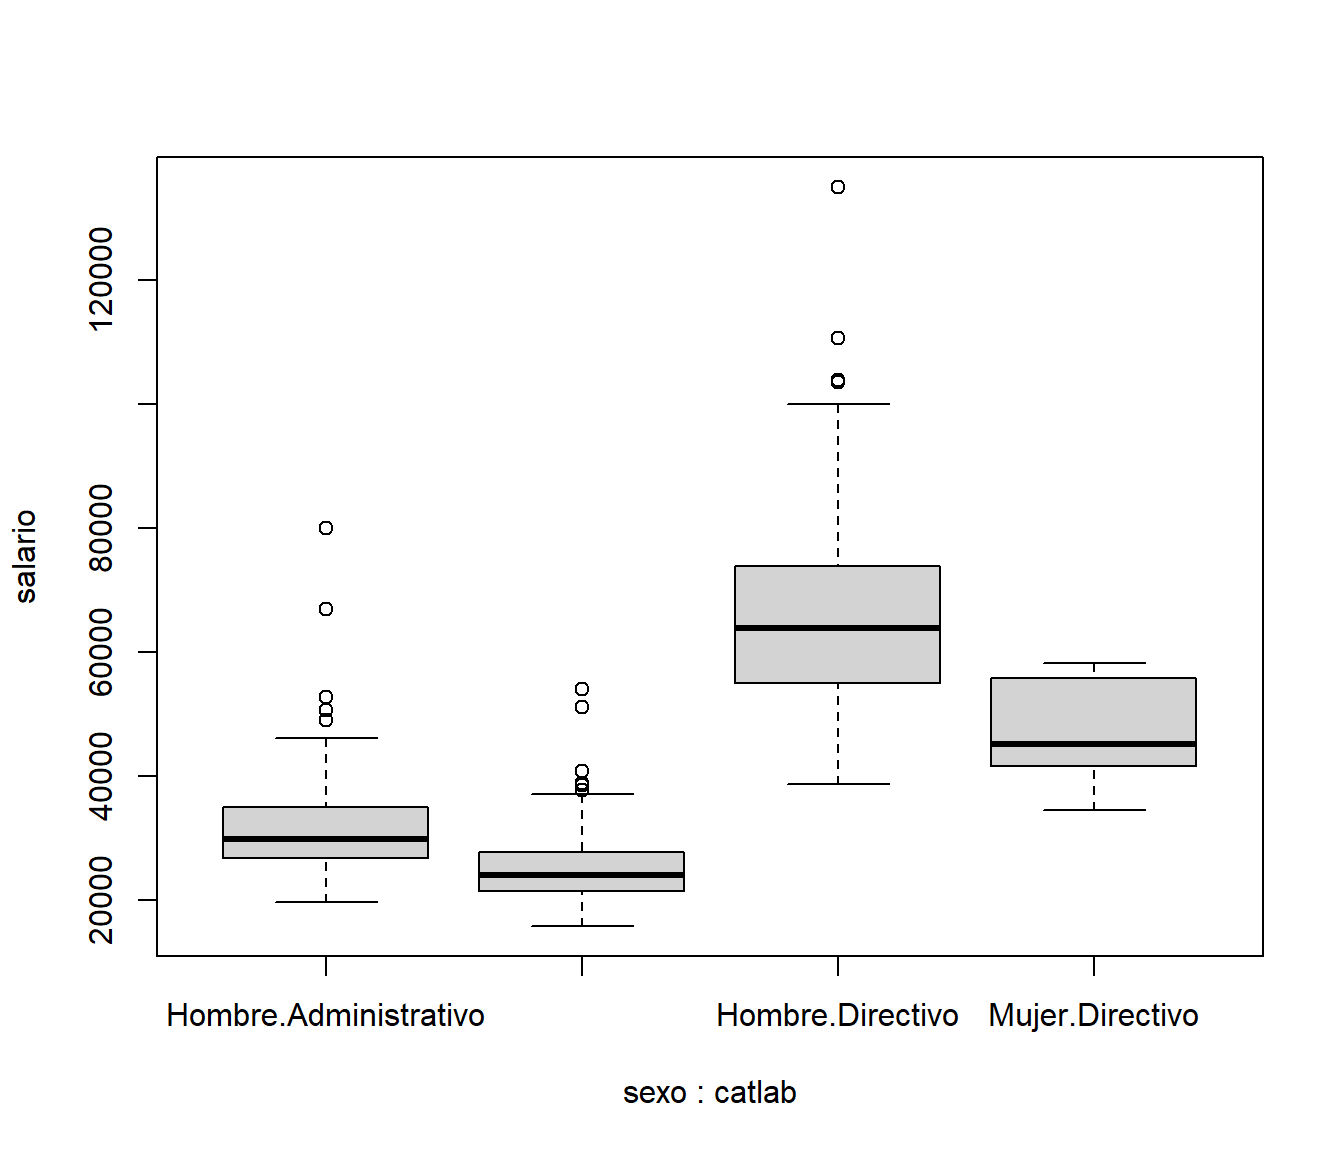
\includegraphics[width=0.8\linewidth]{10_tidyverse_files/figure-latex/unnamed-chunk-1-1} \end{center}

\hypertarget{referencias}{%
\chapter*{Referencias}\label{referencias}}
\addcontentsline{toc}{chapter}{Referencias}

Fernández-Casal R., Costa J. y Oviedo de la Fuente, M. (2021). \emph{\href{https://rubenfcasal.github.io/aprendizaje_estadistico}{Aprendizaje Estadístico}}. \href{https://github.com/rubenfcasal/aprendizaje_estadistico}{github}.

Fernández-Casal R., Roca-Pardiñas J., Costa J. y Oviedo-de la Fuente M. (2023). \emph{\href{https://rubenfcasal.github.io/intror}{Introducción al Análisis de Datos con R}}. ISBN: 978-84-09-41823-7. \href{https://github.com/rubenfcasal/intror}{github}.

Grolemund, G. (2014). \emph{\href{https://rstudio-education.github.io/hopr}{Hands-on programming with R: Write your own functions and simulations}}, \href{http://shop.oreilly.com/product/0636920028574.do}{O'Reilly}.

Kuhn, M. y Silge, J. (2022). \emph{\href{https://www.tmwr.org}{Tidy Modeling with R}}. \href{https://amzn.to/35Hn96s}{O'Reill}.

Matloff, N. (2011). \emph{The art of R programming: A tour of statistical software design}, \href{https://www.nostarch.com/artofr.htm}{No Starch Press}.

Wickham, H. (2015). \emph{\href{http://r-pkgs.had.co.nz/}{R packages: organize, test, document, and share your code}} (actualmente 2ª edición en desarrollo con H. Bryan), \href{http://shop.oreilly.com/product/0636920034421.do}{O'Reilly, 1ª edición}.

Wickham, H. (2019). \emph{\href{https://adv-r.hadley.nz/}{Advanced R, 2ª edición}}, \href{https://www.amazon.com/dp/0815384572}{Chapman \& Hall}, \href{http://adv-r.had.co.nz/}{1ª edición.}.

Wickham, H., y Grolemund, G. (2016). \emph{\href{http://r4ds.had.co.nz}{R for data science: import, tidy, transform, visualize, and model data}}, \href{https://es.r4ds.hadley.nz}{online-castellano}, \href{http://shop.oreilly.com/product/0636920034407.do}{O'Reilly}.

NOTA: En la bibliografía complementaria se incluyen algunas de estas referencias, y una selección de libros en abierto, organizados por temas.

\hypertarget{bibliografuxeda-por-temas}{%
\section*{Bibliografía por temas}\label{bibliografuxeda-por-temas}}
\addcontentsline{toc}{section}{Bibliografía por temas}

\textbf{\emph{En preparación\ldots{}}}

A continuación se muestra una selección de \textbf{\emph{libros en abierto}} que considero que pueden resultar de utilidad.
Para referencias adicionales recomiendo consultar:

\begin{itemize}
\tightlist
\item
  Baruffa, O. (2022). \emph{\href{https://www.bigbookofr.com}{Big Book of R}}: Your last-ever bookmark (hopefully\ldots).
\end{itemize}

\hypertarget{iniciaciuxf3n-a-la-programaciuxf3n-en-r}{%
\subsection*{Iniciación a la programación en R}\label{iniciaciuxf3n-a-la-programaciuxf3n-en-r}}
\addcontentsline{toc}{subsection}{Iniciación a la programación en R}

\begin{itemize}
\item
  Wickham, H., y Grolemund, G. (2016). \emph{\href{http://r4ds.had.co.nz}{R for data science: import, tidy, transform, visualize, and model data}}, \href{https://es.r4ds.hadley.nz}{online-castellano}, \href{http://shop.oreilly.com/product/0636920034407.do}{O'Reilly}.
\item
  Grolemund, G. (2014). \emph{\href{https://rstudio-education.github.io/hopr}{Hands-on programming with R: Write your own functions and simulations}}, \href{http://shop.oreilly.com/product/0636920028574.do}{O'Reilly}.
\item
  Fernández-Casal R., Roca-Pardiñas J., Costa J., y Oviedo de la Fuente, M. (2022). \emph{\href{https://rubenfcasal.github.io/intror}{Introducción al Análisis de Datos con R}}. \href{https://github.com/rubenfcasal/intror}{github}.
\item
  Peng, R.D. (2022). \emph{\href{https://bookdown.org/rdpeng/rprogdatascience}{R Programming for Data Science}}, \href{https://leanpub.com/rprogramming}{Leanpub}.
\end{itemize}

\hypertarget{programaciuxf3n-avanzada-en-r}{%
\subsection*{Programación avanzada en R}\label{programaciuxf3n-avanzada-en-r}}
\addcontentsline{toc}{subsection}{Programación avanzada en R}

\begin{itemize}
\item
  Wickham, H. (2019). \emph{\href{https://adv-r.hadley.nz/}{Advanced R, 2ª edición}}, \href{https://www.amazon.com/dp/0815384572}{Chapman \& Hall}, \href{http://adv-r.had.co.nz/}{1ª edición.}.
\item
  Wickham, H. (2015). \emph{\href{http://r-pkgs.had.co.nz/}{R packages: organize, test, document, and share your code}} (actualmente 2ª edición en desarrollo con H. Bryan), \href{http://shop.oreilly.com/product/0636920034421.do}{O'Reilly, 1ª edición}.
\end{itemize}

\hypertarget{regresiuxf3n-y-aprendizaje-estaduxedstico}{%
\subsection*{Regresión y aprendizaje estadístico}\label{regresiuxf3n-y-aprendizaje-estaduxedstico}}
\addcontentsline{toc}{subsection}{Regresión y aprendizaje estadístico}

\begin{itemize}
\item
  Fernández-Casal R., Costa J. y Oviedo de la Fuente, M. (2021). \emph{\href{https://rubenfcasal.github.io/aprendizaje_estadistico}{Aprendizaje Estadístico}}. \href{https://github.com/rubenfcasal/aprendizaje_estadistico}{github}.
\item
  Kuhn, M., y Silge, J. (2022). \emph{\href{https://www.tmwr.org}{Tidy Modeling with R}}, \href{https://www.oreilly.com/library/view/tidy-modeling-with/9781492096474}{O'Reilly}.
\item
  Fernández-Casal R., Cao R. y Costa J. (2023). \emph{\href{https://rubenfcasal.github.io/simbook}{Técnicas de Simulación y Remuestreo}} (\href{https://github.com/rubenfcasal/simbook}{github}). La anterior edición (Fernández-Casal R. y Cao R., 2022, \emph{Simulación Estadística}) está disponible en la rama \emph{\href{https://github.com/rubenfcasal/simbook/tree/primera_edicion}{primera\_edicion}}.
\end{itemize}

\hypertarget{datos-temporales-y-espaciales}{%
\subsection*{Datos temporales y espaciales}\label{datos-temporales-y-espaciales}}
\addcontentsline{toc}{subsection}{Datos temporales y espaciales}

\begin{itemize}
\item
  Fernández-Casal R. y Cotos-Yáñez T.R. (2021). \emph{\href{https://rubenfcasal.github.io/estadistica_espacial}{Estadística Espacial con R}}. \href{https://github.com/rubenfcasal/estadistica_espacial}{github}.
\item
  Hyndman, R.J., y Athanasopoulos, G. (2021). \emph{\href{https://otexts.com/fpp3}{Forecasting: principles and practice}}. \href{https://www.amazon.es/dp/0987507133}{OTexts}.
\item
  Lovelace, R., Nowosad, J., y Muenchow, J. (2019). \emph{\href{https://geocompr.robinlovelace.net}{Geocomputation with R}}. \href{https://www.routledge.com/9781138304512}{CRC}.
\item
  Moraga, P. (2019). \emph{\href{https://www.paulamoraga.com/book-geospatial}{Geospatial health data: Modeling and visualization with R-INLA and shiny}}, \href{https://www.routledge.com/9780367357955}{CRC}.
\item
  Pebesma, E., y Bivand, R. (2021). \emph{\href{https://keen-swartz-3146c4.netlify.app}{Spatial Data Science}}.
\end{itemize}

\hypertarget{datos-faltantes}{%
\subsection*{Datos faltantes}\label{datos-faltantes}}
\addcontentsline{toc}{subsection}{Datos faltantes}

\begin{itemize}
\tightlist
\item
  Buuren, S. (2018). \emph{\href{https://stefvanbuuren.name/fimd}{Flexible Imputation of Missing Data}}, \href{}{Chapman \& Hall}.
\end{itemize}

\hypertarget{rmarkdown}{%
\subsection*{Rmarkdown}\label{rmarkdown}}
\addcontentsline{toc}{subsection}{Rmarkdown}

\begin{itemize}
\tightlist
\item
  Fernández-Casal, R. y Cotos-Yáñez, T.R. (2018). \emph{\href{https://rubenfcasal.github.io/bookdown_intro}{Escritura de libros con bookdown}}, \href{https://github.com/rubenfcasal/bookdown_intro}{github}. Incluye un apéndice con una \href{https://rubenfcasal.github.io/bookdown_intro/rmarkdown.html}{Introducción a RMarkdown}.
\end{itemize}

\hypertarget{manuales-oficiales}{%
\subsection*{Manuales oficiales}\label{manuales-oficiales}}
\addcontentsline{toc}{subsection}{Manuales oficiales}

\url{https://cran.r-project.org/manuals.html}

\begin{itemize}
\item
  \href{http://colinfay.me/intro-to-r/}{Intro to R}
\item
  \href{http://colinfay.me/r-data-import-export/}{R Data Import/Export}
\item
  \href{http://colinfay.me/r-installation-administration/}{R Installation and Administration}
\item
  \href{http://colinfay.me/writing-r-extensions/}{Writing R extensions}
\item
  \href{http://colinfay.me/r-language-definition/}{The R language definition}
\item
  \href{http://colinfay.me/r-internals/}{R Internals}
\end{itemize}

\hypertarget{links}{%
\section*{Enlaces}\label{links}}
\addcontentsline{toc}{section}{Enlaces}

\textbf{\emph{Repositorio}}: \href{https://github.com/rubenfcasal/book_notasr}{rubenfcasal/book\_notasr}

\textbf{\emph{Recursos para el aprendizaje de R}}: En este \href{https://rubenfcasal.github.io/post/ayuda-y-recursos-para-el-aprendizaje-de-r}{post} se muestran algunos recursos que pueden ser útiles para el aprendizaje de R y la obtención de ayuda.

\href{https://bookdown.org}{\textbf{\emph{Bookdown}}}:

\begin{itemize}
\item
  \href{https://rubenfcasal.github.io/book_notasr/}{Notas de programación en R}
\item
  \href{https://rubenfcasal.github.io/bookdown_intro/rmarkdown.html}{Introducción a RMarkdown}.
\end{itemize}

\href{https://posit.co}{\textbf{\emph{Posit (RStudio)}}}

\begin{itemize}
\item
  \href{https://posit.co/blog}{Blog}
\item
  \href{https://posit.co/resources/videos}{Videos}
\item
  \href{https://posit.co/resources/cheatsheets}{Chuletas (Cheatsheets)}
\item
  \href{https://www.tidyverse.org/}{\textbf{\emph{tidyverse}}}:

  \begin{itemize}
  \item
    \href{https://dplyr.tidyverse.org}{dplyr}
  \item
    \href{https://tibble.tidyverse.org}{tibble}
  \item
    \href{https://tidyr.tidyverse.org}{tidyr}
  \item
    \href{https://stringr.tidyverse.org}{stringr}
  \item
    \href{https://readr.tidyverse.org}{readr}
  \item
    \href{https://solutions.posit.co/connections/db}{Best Practices in Working with Databases}
  \end{itemize}
\item
  \href{https://www.tidymodels.org}{tidymodels}
\item
  \href{https://spark.rstudio.com/}{sparklyr}
\item
  \href{http://shiny.rstudio.com}{shiny}
\end{itemize}

  \bibliography{book.bib,packages.bib}

\end{document}
